\documentclass[11pt]{article}
\usepackage{hyperref}
\usepackage{amsthm}
\usepackage{amsmath}
\usepackage{amsfonts}
\usepackage{tikz}
\usepackage{ wasysym }

\newtheorem{example}{Example}


\author{}
\title{}

\begin{document}
\pagenumbering{roman}
%\maketitle
{\Large
%Change Document name to: Graded Homework 1\_Jacob\_Nicholas
\noindent NAME:  Nicholas Jacob\\ 
EMAIL: \href{mailto: nicholascjacobphd@gmail.com}{nicholas.c.jacob-1@ou.edu}\\
STUDENT ID: \# 113578513\\
Final Project\\
COURSE: CS/DSA 4513 DATABASE MANAGEMENT\\ 
SECTION: ONLINE\\SEMESTER: FALL 2023\\
INSTRUCTOR:  DR. LE GRUENWALD\\
 SCORE:}

\newpage
\tableofcontents
\newpage
\pagenumbering{arabic}
\setcounter{page}{1}

\section{ER Diagram}
Here is my ER diagram

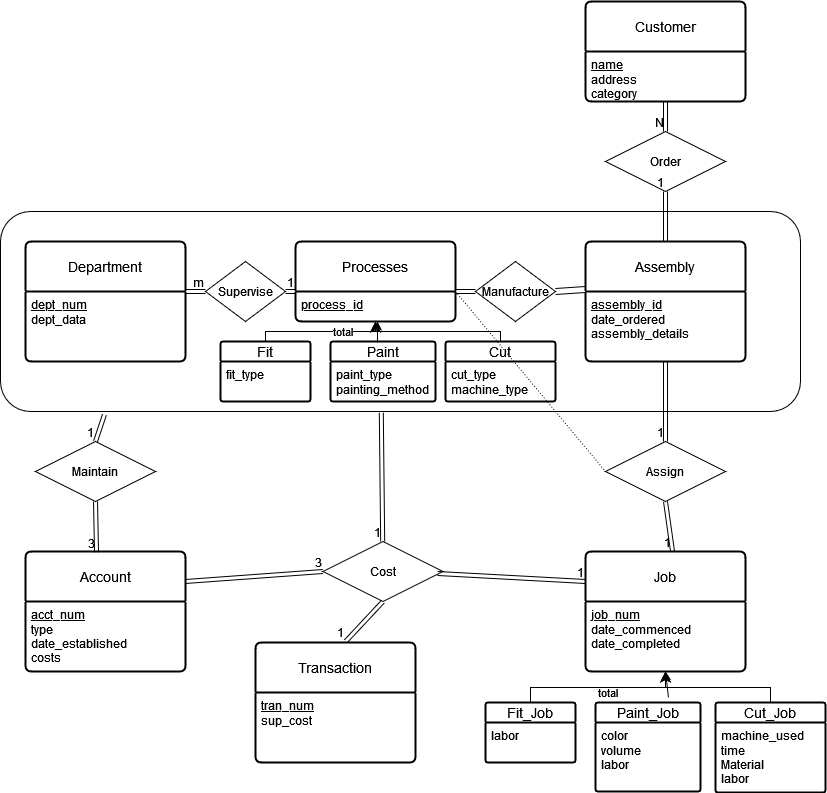
\includegraphics[width=\textwidth]{Project.png}
\newpage

\section{Relational Database Schema}

\indent Here are my schema:

Process(\underline{process\_id},process\_data)

Assemblies(\underline{ass\_id},ass\_details)

Create(\underline{process\_id},\underline{ass\_id})

Customer(\underline{name},address, category)

Orders(\underline{name},\underline{ass\_id})

Department(\underline{dept\_num},dept\_data)

Supervises(\underline{dept\_num},\underline{process\_id})



\end{document}